%!TeX root =main.tex
%!TEX program = XeLaTeX
% !Mode:: "TeX:UTF-8"

\section{牛顿运动定律}

\subsection{牛顿第三定律}
\begin{enumerate}[(a)]
%%%%%%  1.1 题  %%%%%%%%%%%%%%
	\item
	他可以一只脚放松,另一只脚用力向后蹬,整个人就可以向前滑动,持续这样,就可以到达边缘。
%%%%%%  1.2 题  %%%%%%%%%%%%%%
	\item
	当脚向后蹬的时候,学生给了地面一个向后下方的作用力$\bm{F}$,根据“牛顿第三定律”,地面也会给学生一个相等大小,但是方向向前的作用力$\bm{F_1} = -\bm{F}$。根据“牛顿第二定律”,质量为$m$的学生在$\bm{F_1}$的作用下得到一个加速度$\bm{a_1} = \frac{\bm{F_1}}{m}$,开始向边缘运动,而地面也会有一个加速度$\bm{a} = \frac{\bm{F}}{M}$,因为$M \to \infty$,所以$\bm{F} \to 0$,所以地面没动,人向边缘滑去。
\end{enumerate}
%%%
%%%
%%%
%%%
%%%
\subsection{}
\label{subsec_3.2}
{\bfseries 证明1:}设O点与P点的水平距离为$x$,P点离地面高度为$y$,子弹速度为$\bm{v}$,$\bm{v}$与水平方向的夹角为$\theta$,重力加速度为$\bm{g}$,则子弹飞过距离$x$ 所需的时间$t$满足
\[
t = \frac{x}{v_x} = \frac{x}{v\sin\theta} = \frac{x}{v \frac{x}{\sqrt{x^2+y^2}}}
\]
在这段时间$t$内,靶体在做自由落体运动,子弹在做竖直上抛运动,靶体距离地面的高度$h$,子弹离地面的高度$H$分别满足
\[
\begin{aligned}
& h = y-\frac{1}{2}gt^2, \\
& H = v_yt - \frac{1}{2}gt^2
\end{aligned}
\]
因为枪是瞄准P点的,因此,子弹初速度的水平分量$v_x$和竖直分量$v_y$满足关系
\[
\frac{v_y}{v_x} = \frac{y}{x}
\]
将$t,\;v_x,\;v_y$分别代入$h,\,\;H$的表达式中,得到
\[
h = y-\frac{1}{2}g \frac{x^2+y^2}{v^2} = H
\]
即无论子弹的速度$\bm{v}$取值为多少,恒有$h = H$。

{\bfseries 证明2:}我们以靶体为参考系,此时,子弹与靶体间不存在相对加速度,两者的相对运动变为:子弹以速度$\bm{v}$匀速飞向静止的靶体。因此,只要子弹瞄准靶体,最终两者会相遇。
%%%
%%%
%%%
%%%
%%%
\subsection{接球游戏的顶棚高度}
因为球的运动轨迹是开口向下的抛物线,根据题意,孩子们能完成这个游戏的充分条件是抛物线的顶点不能超过顶棚(如下图(\ref{3_3a})所示)。
%%%%以下画图时间
\begin{figure}[htbp]
	\centering
	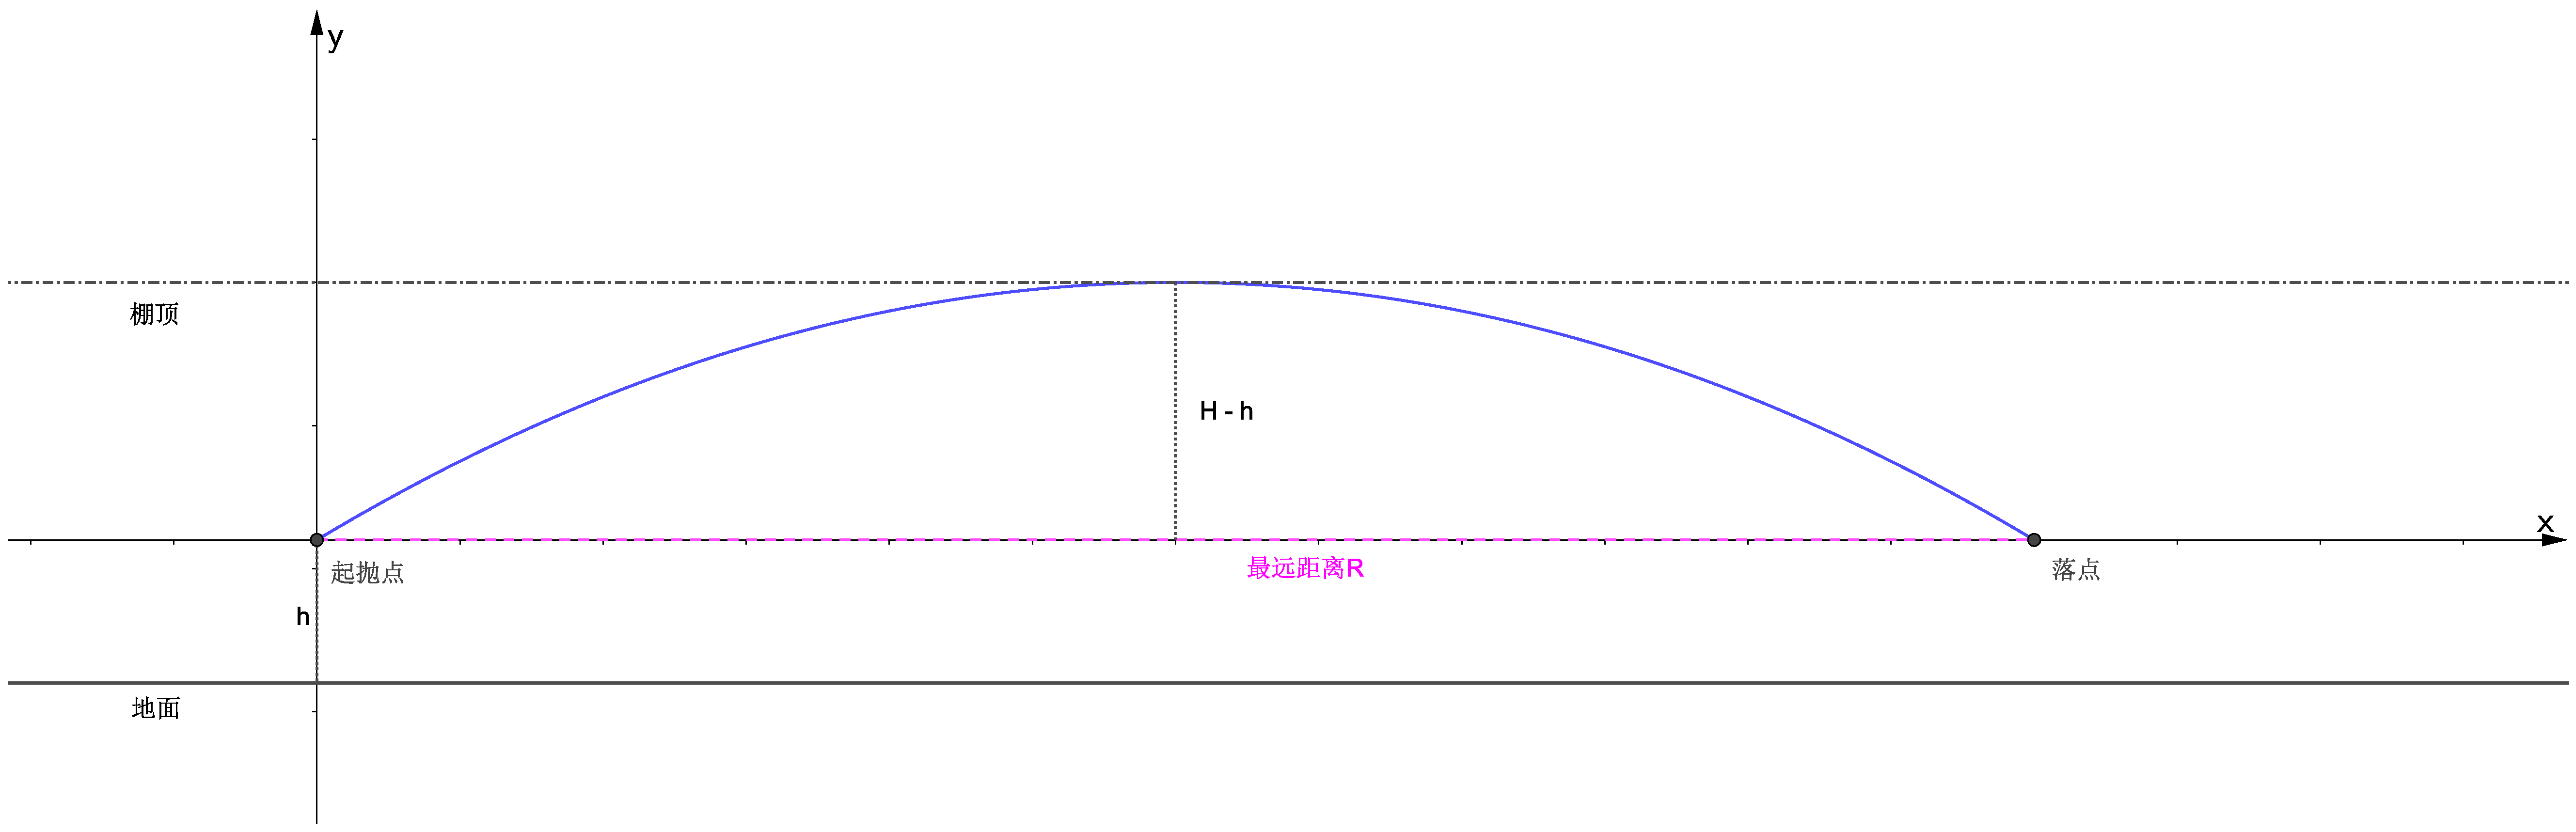
\includegraphics[width=0.8\textwidth]{3_3a.eps}
	\caption{}
	\label{3_3a}
\end{figure}

\noindent
而抛体的运动函数为
\[
y - \left(y_0 + \frac{v_0^2\sin\theta}{2g}\right) = - \frac{g}{2v_0^2\cos^2\theta}\left[x - \left(x_0 + \frac{v_0^2\sin	\theta \cos\theta}{g}\right)\right]^2.
\]
这条抛物线的顶点在
\[
\begin{aligned}
&x_1 = x_0 + \frac{v_0^2\sin \theta\cos \theta}{g}\;, \\
&y_1 = y_0 + \frac{v_0^2 \sin^2 \theta}{2g}\;.
\end{aligned}
\]

不妨建立如图(\ref{3_3a})所示的直角坐标系,假设两个孩子相距的最远距离为$R$,孩子扔球的初始速度大小为$v_0$,与地面的夹角为$\theta$,则有$(x_0, y_0) = (0, 0),\;(x_1,y_1) = (\frac{R}{2},H-h)$,将这些条件代入上述的顶点公式中有:
\[
\begin{aligned}
&\frac{R}{2} = \frac{v_0^2\sin \theta\cos \theta}{g}\;, \\
&H-h = \frac{v_0^2 \sin^2 \theta}{2g}\;.
\end{aligned}
\]

\newpage
\noindent
{\bfseries 解法一(错误解法):}\par
设$l = \sqrt{\frac{R}{2}^2 +(H-h)^2}$,则
\[
\begin{aligned}
&\sin \theta = \frac{H-h}{l}\;, \\
&\cos \theta = \frac{(\frac{R}{2})}{l} = \frac{R}{2l}\;,\\
& \sin 2\theta = 2\sin \theta \cos \theta = \frac{(H-h)R}{l^2}.
\end{aligned}
\]
因此,{\bfseries\textcolor{red}{!!!此处出现矛盾,书上给出的参考答案是第二种。}}
\[
\begin{aligned}
&R = \frac{v_0^2}{g}\frac{(H-h)R}{l} \Rightarrow R = 4\sqrt{\frac{v_0^2}{g}(H-h) - (H-h)^2}\;,\\
&H-h = \frac{v_0^2}{2g}\left(\frac{H-h}{l}\right)^2 \Rightarrow R = 4\sqrt{\frac{v_0^2}{2g}(H-h) - (H-h)^2}\;.
\end{aligned}
\]
{\bfseries\textcolor{red}{警告!!!这种解法有问题!如图(\ref{3_3b})所示,其中的错误是在:将球抛出的初始速度与水平方向的夹角和最高点与最远距离的中点的夹角混淆了!}}


%%%%以下画图时间
\begin{figure}[htbp]
	\centering
	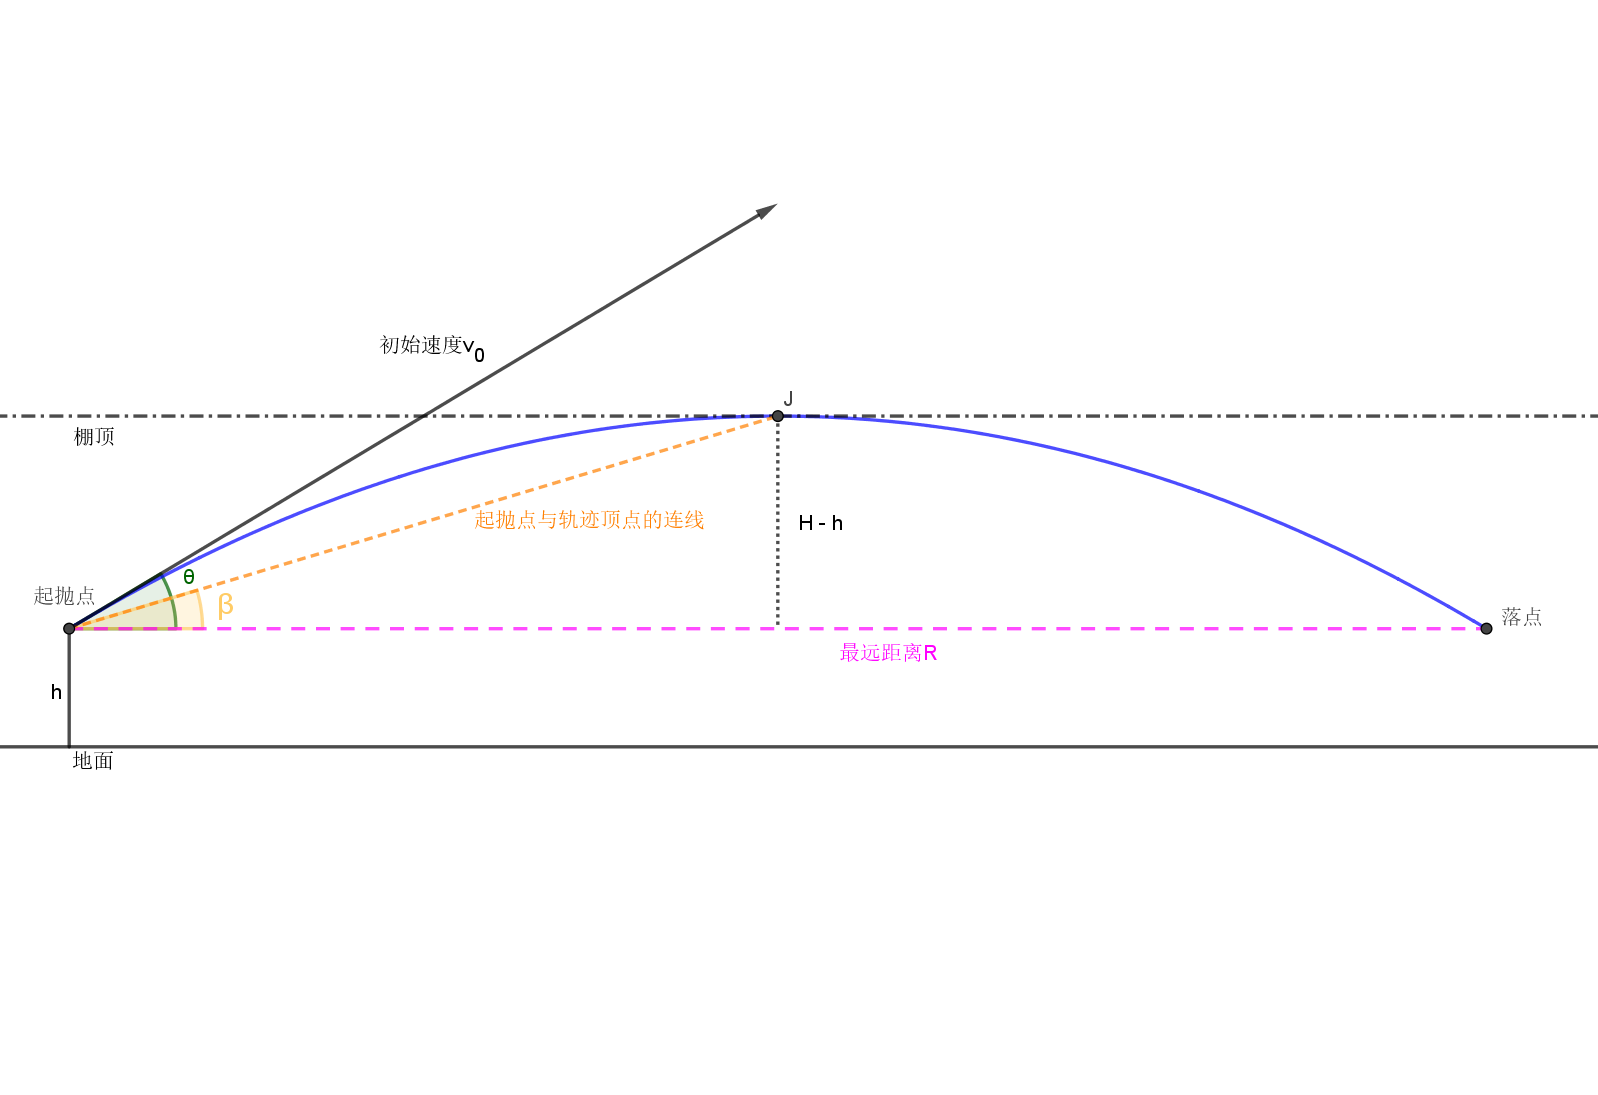
\includegraphics[width=0.8\textwidth]{3_3b.png}
	\caption{}
	\label{3_3b}
\end{figure}

\newpage
\noindent
{\bfseries 解法二:}\par
如图(\ref{3_3c})所示,

%%%%以下画图时间
\begin{figure}[htbp]
	\centering
	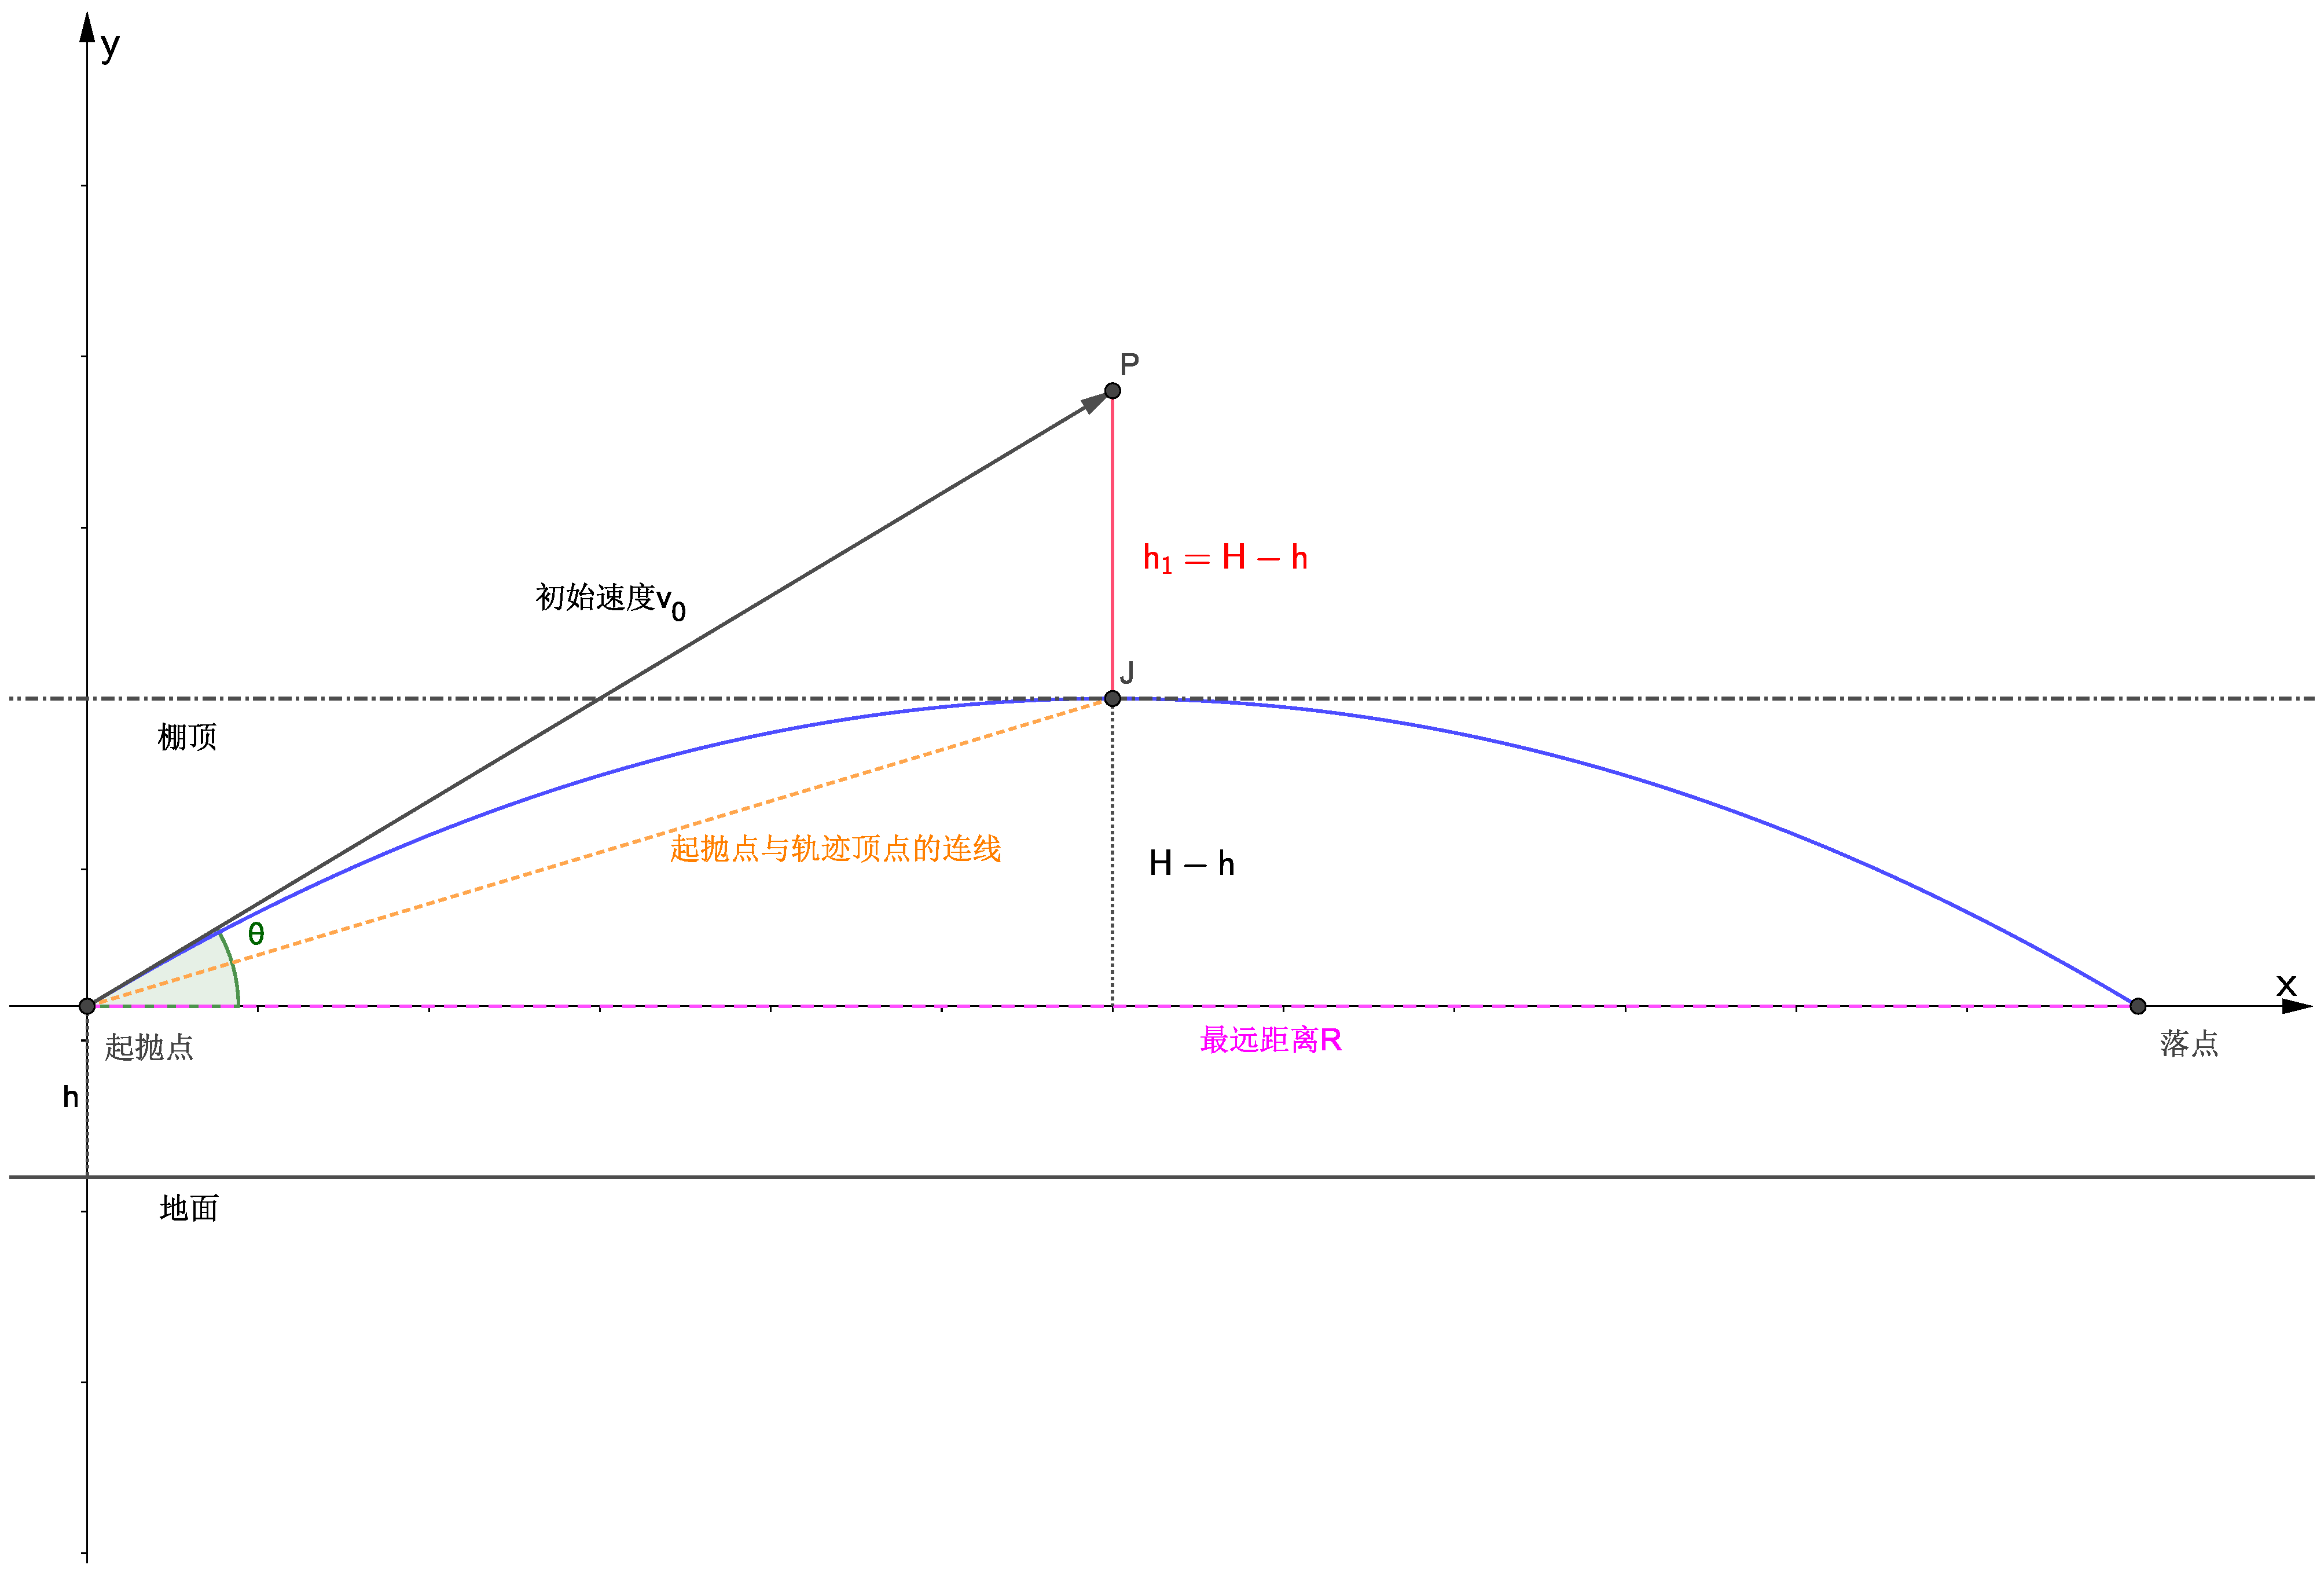
\includegraphics[width=0.8\textwidth]{3_3c.eps}
	\caption{}
	\label{3_3c}
\end{figure}

\noindent
根据运动公式
\[
\begin{aligned}
& 0 - v_y = -gt\;,\\
& 0^2 - v_y^2 = 2g(H-h)
\end{aligned}
\]
可以得到
\[
v_y = gt = \sqrt{2g(H-h)} \Rightarrow t = \sqrt{\frac{2(H-h)}{g}}
\]
根据{\bfseries 题\ref{subsec_3.2}}可以知道,当物体1以任意速度开始做斜上抛运动时,如果在初始速度的方向上有物体2立刻做自由落体运动,那么最终两个物体会在物体1的抛物线轨迹上相遇。由此我们可以知道,图(\ref{3_3c})中,点P到抛物线的顶点J的距离$l_{\text{PJ}}$应该满足
\[
l_{\text{PJ}} = \frac{1}{2}gt^2 = \frac{g}{2} \cdot \frac{2(H-h)}{g} = H - h
\]
由此我们可以得到
\[
\begin{aligned}
& \sin \theta = \frac{2(H - h)}{\sqrt{[2(H - h)]^2 + (\frac{R}{2})^2}}\;,\\
& \cos \theta = \frac{(\frac{R}{2})}{\sqrt{[2(H - h)]^2 + (\frac{R}{2})^2}}\;.
\end{aligned}
\]
将得到的$\sin \theta\;,\cos \theta$分别代入开始得到$R$和$H - h$的表达式中得到
\[
\begin{aligned}
& R = \frac{2v_0^2}{g} \cdot \frac{(H-h)R}{[2(H - h)]^2 + (\frac{R}{2})^2} \Rightarrow R = 4\sqrt{\frac{v_0^2}{2g}(H-h) - (H-h)^2}\;,\\
& H-h = \frac{v_0^2}{2g} \cdot \left(\frac{2(H - h)}{\sqrt{[2(H - h)]^2 + (\frac{R}{2})^2}}\right)^2 \Rightarrow R = 4\sqrt{\frac{v_0^2}{2g}(H-h) - (H-h)^2}\;.
\end{aligned}
\]

\noindent
对于第2问,令$h_0 = H - h$,则
\[
\begin{aligned}
& R = 4\sqrt{\frac{v_0^2}{2g}h_0 - h_0^2}\;,\\
& R' = \frac{\mathrm{d}R}{\mathrm{h_0}} = 4\times \frac{1}{2}\frac{1}{\sqrt{\frac{v_0^2h_0}{2g} - h_0^2}}(\frac{v_0^2}{2g} - 2h_0)\;.
\end{aligned}
\]
令$R'(h_0) = 0$,可以解得$h_0 = \frac{v_0^2}{4g}$,此时$R$有最大值
\[
R = 4\sqrt{ \frac{v_0^2}{2g}\cdot\frac{v_0^2}{4g} - ( \frac{v_0^2}{4g})^2} = \frac{v_0}{g}
\]
此处$R$的最大值表示,在不受棚顶高度限制的情况下孩子在以速度$v_0$将球抛出时所能达到的最远距离,因此$h_0 = H - h$ 表示,在没有棚顶高度限制,并且球达到最远距离的情况下球所能达到的最大高度。
%%%
%%%
%%%
%%%
%%%
\subsection{向上发射}
\begin{enumerate}[(a)]
%%%%%% 4.1题  %%%%%%%%%%%%%%
	\item
	设子弹最高可以到达的高度是$h$,子弹速度为$v$,重力加速度$g = 10\;\text{m/s}^2$,,则
	\[
		\begin{aligned}
			&0 - v = -gt \Rightarrow t = \frac{v}{g} = 3\,\text{s}\;,\\
			&h = vt - \frac{1}{2}gt^2 = 30 \times 3 - 0.5 \times 10 \times 3^2 = 45\;\text{m}\;.
		\end{aligned}
	\]
	因为子弹上升和下降的过程是对称的,因此,每一颗子弹在空中停留的时间均为6s,不妨设此人在$t = 0\,\text{s}$时射出第一发子弹,则在$t = 6\,\text{s}$时这一颗子弹刚好回到地面。根据题意,此人每隔一秒发射一颗子弹,因此,最终(第6秒之后)空中子弹数量为6,在第6秒之前,子弹数量逐渐增加,如下表(\ref{3_3ta})所示。
	\begin{table}[htbp]
		\centering
		\begin{tabular}{c|cccccccccc}
		\hline
		\text{时间/s} & 0 & 1 & 2 & 3 & 4 & 5 & 6 & 7 & ... & n \\
		\hline
		\text{子弹数量/颗} & 1 & 2 & 3 & 4 & 5 & 6 & 6 & 6 & ... & 6 \\
		\hline
		\end{tabular}
		\caption{}
		\label{3_3ta}
	\end{table}
%%%%%% 4.2题  %%%%%%%%%%%%%%
	\item 
	当第一颗子弹b1(在第0秒发射)开始下落时,首先遇到的是在第1秒发射的子弹b2。在此之前,b1运动时间为3s,刚好到达轨迹最高点并开始转做自由落体运动,b2运动时间为$t_2 = 2$s,仍在以速度$v_20$竖直上抛的过程中,以此为时间参考点,因为运动过程对称,因此两者相遇时速度大小为$v_2$,相遇的时间$t_{02}$满足
	\[
		\begin{aligned}
			& v_{20} - v = -gt_2 \\
			& v_2 - v_{20} = -gt_{02} \\
			& -v_2 = -gt_{02}
		\end{aligned}
	\]
	解得:
	\[
		t_{02} = \frac{v-2g}{2g} = 0.5\;\text{s}
	\]
	因此,b1和b2相遇的地方离地面高度$h_2 =h - \frac{1}{2}gt_{02}^2 = 43.75$m。
	b1接下来遇到的子弹是在第2秒发射的子弹b3,在第3秒发射的子弹b4,在第4秒发射的子弹b5,在第5秒发射的子弹b6,根据上面一样的做法,可以分别得到各自相遇的时间和离地面的高度。结果如下表(\ref{3_3tb})所示。
	\begin{table}[htbp]
		\centering
		\begin{tabular}{|c|c|c|c|c|c|c|}
		\hline
		\text{与b1相遇的子弹} & b2 & b2 & b3 & b4 & b5 & b6 \\
		\hline
		\text{时间/s} & 0.5 & 1 & 1.5 & 2 & 2.5 & 3 \\
		\hline
		\text{离地面高度/m} & 43.75 & 40 & 33.75 & 25 & 13.75 & 0 \\
		\hline
		\end{tabular}
		\caption{}
		\label{3_3tb}
	\end{table}
\end{enumerate}
%%%
%%%
%%%
%%%
%%%
\subsection{两个斜面上的摩擦}
设$M_1$受到的重力为$G_1 = M_1g$,摩擦力为$f_1 = \mu_1 G_1\cos \theta_1$,$M_2$受到的重力为$G_2 = M_2g$,摩擦力为$f_2 = \mu_2 G_2\cos \theta_2$,绳子拉力为$T$。
\begin{enumerate}[(a)]
%%%%%% 5.1题  %%%%%%%%%%%%%%	
	\item 
	当$M_1$刚要沿平面下滑时,分别对$M_1$和$M_2$进行受力分析,可以知道,$M_1$刚要下滑,摩擦力和运动趋势相反,即沿斜面向上;而对于$M_2$,因为$M_1$已经要开始滑动,所以$M_2$的状态应当是被$M_1$拉着将要向上走,因此$M_2$的摩擦力是沿斜面向下,所以可以有以下关系:
	\[
		\begin{aligned}
			f_1 & = G_1\sin \theta_1 - T \;,\\
			f_2 & = T - G_2\sin \theta_2
		\end{aligned}
		\]
	将相关的表达式代入后将两式相加,并整理可得:
	\[
		\frac{M_1}{M_2} = \frac{\mu_2\cos\theta_2 + \sin\theta_2}{\sin\theta_1 - \mu_1\cos\theta_1}
		\]
	这就是在条件“$M_1$刚要沿平面下滑时”各个物理量之间要满足的关系。
%%%%%% 5.2题  %%%%%%%%%%%%%%
	\item
	当当$M_2$刚要沿平面下滑时,可以对$M_1$和$M_2$分别进行跟题(a)一样的受力分析,并得出以下关系:
	\[
		\begin{aligned}
			f_1 & = T - G_1\sin \theta_1 \;,\\
			f_2 & = G_2\sin \theta_2 - T
		\end{aligned}
		\]
	将相关的表达式代入后将两式相加,并整理可得:
	\[
		\frac{M_1}{M_2} = \frac{\mu_2\cos\theta_2 - \sin\theta_2}{\sin\theta_1 + \mu_1\cos\theta_1}
		\]
	这就是在条件“$M_2$刚要沿平面下滑时”各个物理量之间要满足的关系。
\end{enumerate}

%%%%以下画图时间




%%%
%%%
%%%
%%%
%%%
\subsection{摩擦力不等于$\mu Mg$}
\begin{enumerate}[(a)]
	\item
	根据题意有
	\[
		F\sin \theta < \mu (Mg + F\cos\theta) \Rightarrow \sin\theta - \mu \cos\theta < \frac{\mu Mg}{F}
		\]
	令$f(\theta) = \sin\theta - \mu \cos\theta, (0 \leqslant \theta \leqslant \frac{\pi}{2})$,则$f'(\theta) = \cos\theta + \mu \sin\theta > 0$恒成立,即$f(\theta)$在定义域内是单调递增的,最大值
	\item
	1+1
\end{enumerate}
%%%
%%%
%%%
%%%
%%%
\subsection{摩擦力不等于$\mu Mg$}
%%%
%%%
%%%
%%%
%%%
\subsection{摩擦力不等于$\mu Mg$}
%%%
%%%
%%%
%%%
%%%
\subsection{摩擦力不等于$\mu Mg$}
%%%
%%%
%%%
%%%
%%%
\subsection{摩擦力不等于$\mu Mg$}
%%%
%%%
%%%
%%%
%%%
\subsection{摩擦力不等于$\mu Mg$}
%%%
%%%
%%%
%%%
%%%
\subsection{摩擦力不等于$\mu Mg$}
